% Основной текст отчёта: постановка задачи, реализация, результаты

\section{Постановка задачи}
Для данной таблицы значений функции построить методом наименьших квадратов линейную и квадратичную полиномиальные модели, вычислить наилучшие среднеквадратические отклонения.

Функция $y = f(x)$ задана таблицей 1. Требуется построить её аналитическое приближение. Для этого по данным таблицы находится функция $y = g(x)$, аппроксимирующая исходную, т.е. удовлетворяющая условию $g(x_i) \approx y_i, i = 1,\dots,n$.

Аппроксимирующая функция строится из условия минимума среднеквадратического отклонения:
\[
\delta^{(2)}(g) = \sqrt{\frac{1}{n} \sum_{i=1}^{n} (y_i - g(x_i))^2} \to \min.
\]

В данной работе аппроксимация проводится в классе алгебраических полиномов степени $m$:
\[
P_m(x) = a_0 + a_1 x + \dots + a_m x^m.
\]
Коэффициенты $a_0, a_1, \dots, a_m$ находятся из нормальной системы МНК:
\[
\sum_{j=0}^{m} a_j \sum_{i=1}^{n} x_i^{j+k} = \sum_{i=1}^{n} y_i x_i^k, \quad k = 0,\dots,m.
\]

\begin{table}[h]
\centering
\begin{tabular}{|c|cccccccccc|}
\hline
$x_i$ & -0.1 & 0.3 & 0.5 & 0.75 & 0.9 & 1.1 & 1.3 & 1.5 & 1.7 & 1.9 \\
$y_i$ & -0.08 & -0.14 & -0.89 & 0.36 & 0.44 & 0.48 & 0.27 & 0.39 & 0.50 & 0.48 \\
\hline
$x_i$ & 2.1 & 2.3 & 2.5 & 2.7 & 2.9 & 3.1 & 3.3 & 3.5 & 3.7 & 3.9 \\
$y_i$ & 0.69 & 0.50 & 0.31 & 0.37 & 0.43 & 0.33 & 0.31 & 0.09 & 0.08 & 0.03 \\
\hline
\end{tabular}
\caption{Исходные данные функции $y = f(x)$.}
\end{table}

\section{Линейная аппроксимация}
В этом разделе строится полином наилучшего среднеквадратического отклонения степени $m = 1$, то есть линейная аппроксимация $P_1(x) = a_0 + a_1x$.
Нормальная система МНК для её коэффициентов имеет вид:
\[
\left\{
\begin{array}{l}
a_0 n + a_1 \sum_{i=1}^{n} x_i = \sum_{i=1}^{n} y_i, \\
a_0 \sum_{i=1}^{n} x_i + a_1 \sum_{i=1}^{n} x_i^2 = \sum_{i=1}^{n} y_i x_i.
\end{array}
\right.
\]

\subsection{Составление вспомогательной таблицы}
Для подстановки в нормальную систему вычислим необходимые суммы.
На листинге 1 приведён код, вычисляющий суммы:
\begin{lstlisting}[style=pythonstyle,caption={Вычисление вспомогательных сумм}]
import numpy as np

x = np.array([-0.1, 0.3, 0.5, 0.75, 0.9, 1.1, 1.3, 1.5, 1.7, 1.9,
              2.1, 2.3, 2.5, 2.7, 2.9, 3.1, 3.3, 3.5, 3.7, 3.9])
y = np.array([-0.08, -0.14, -0.89, 0.36, 0.44, 0.48, 0.27, 0.39, 0.50,
              0.48, 0.69, 0.50, 0.31, 0.37, 0.43, 0.33, 0.31, 0.09, 0.08, 0.03])

n = len(x)
sx = np.sum(x)
sx2 = np.sum(x**2)
sy = np.sum(y)
sxy = np.sum(x * y)

print(f"n = {n}")
print(f"sum x = {sx:.4f}")
print(f"sum x2 = {sx2:.4f}")
print(f"sum y = {sy:.4f}")
print(f"sum xy = {sxy:.4f}")
\end{lstlisting}

\subsection{Решение нормальной системы}
Подставляя вычисленные суммы при $n = 20$, получаем нормальную систему для линейной аппроксимации:
\[
\left\{
\begin{array}{l}
20 a_0 + 39.8500 a_1 = 4.9500, \\
39.8500 a_0 + 109.1325 a_1 = 11.2185.
\end{array}
\right.
\]

Решаем её с помощью кода, приведённого на листинге 2.

\begin{lstlisting}[style=pythonstyle,caption={Линейная аппроксимация МНК}]
# Нормальная система: A * a = b
A = np.array([[n, sx],
              [sx, sx2]])
b = np.array([sy, sxy])

a0, a1 = np.linalg.solve(A, b)

# Аппроксимирующий полином и отклонение
P1 = a0 + a1 * x
delta1 = np.sqrt(np.sum((y - P1)**2) / n)

print(f"a0 = {a0:.4f}, a1 = {a1:.4f}")
print(f"P1(x) = {a0:.4f} + ({a1:.4f})*x")
print(f"delta2(P1) = {delta1:.4f}")
\end{lstlisting}

Решение нормальной системы даёт коэффициенты:
\[
a_0 = 0.1705, \quad a_1 = 0.0386.
\]
Таким образом, линейная аппроксимирующая функция имеет вид:
\[
P_1(x) = 0.1705 + 0.0386 x.
\]

\subsection{Вычисление наилучшего среднеквадратического отклонения}
Наилучшее среднеквадратическое отклонение вычисляется по формуле:
\[
\delta^{(2)}(P_1) = \sqrt{\frac{1}{n} \sum_{i=1}^{n} (y_i - P_1(x_i))^2}
\]
Подставляем сумму квадратов отклонений $\sum_{i=1}^{n} (y_i - P_1(x_i))^2 = 1.8415$:
\[
\delta^{(2)}(P_1) = \sqrt{\frac{1}{20} \cdot 1.8415} = 0.3034.
\]

\section{Квадратичная аппроксимация}
В этом разделе строится полином наилучшего среднеквадратического отклонения степени $m = 2$, то есть квадратичная аппроксимация $P_2(x) = a_0 + a_1x + a_2x^2$.
Нормальная система МНК для её коэффициентов:
\[
\left\{
\begin{array}{l}
a_0 n + a_1 \sum x_i + a_2 \sum x_i^2 = \sum y_i, \\
a_0 \sum x_i + a_1 \sum x_i^2 + a_2 \sum x_i^3 = \sum y_i x_i, \\
a_0 \sum x_i^2 + a_1 \sum x_i^3 + a_2 \sum x_i^4 = \sum y_i x_i^2.
\end{array}
\right.
\]

\subsection{Дополнительные суммы}
Помимо сумм, найденных в разделе 2, потребуются ещё $\sum x_i^3$, $\sum x_i^4$ и $\sum y_i x_i^2$. Они равны:
\[
\sum x_i^3 = 338.2176, \quad \sum x_i^4 = 1121.7825, \quad \sum y_i x_i^2 = 31.9079.
\]

\subsection{Решение нормальной системы}
Подставляя все суммы, нормальная система принимает вид:
\[
\left\{
\begin{array}{l}
20 a_0 + 39.8500 a_1 + 109.1325 a_2 = 4.9500, \\
39.8500 a_0 + 109.1325 a_1 + 338.2176 a_2 = 11.2185, \\
109.1325 a_0 + 338.2176 a_1 + 1121.7825 a_2 = 31.9079.
\end{array}
\right.
\]

\begin{lstlisting}[style=pythonstyle,caption={Квадратичная аппроксимация МНК}]
sx3 = np.sum(x**3)
sx4 = np.sum(x**4)
sx2y = np.sum(x**2 * y)

# Нормальная система: A * a = b
A = np.array([[n, sx, sx2],
              [sx, sx2, sx3],
              [sx2, sx3, sx4]])
b = np.array([sy, sxy, sx2y])

a0, a1, a2 = np.linalg.solve(A, b)

# Аппроксимирующий полином и отклонение
P2 = a0 + a1 * x + a2 * x**2
delta2 = np.sqrt(np.sum((y - P2)**2) / n)

print(f"a0 = {a0:.4f}, a1 = {a1:.4f}, a2 = {a2:.4f}")
print(f"P2(x) = {a0:.4f} + ({a1:.4f})*x + ({a2:.4f})*x^2")
print(f"delta2(P2) = {delta2:.4f}")
\end{lstlisting}

Решение системы даёт коэффициенты:
\[
a_0 = -0.0988, \quad a_1 = 0.4079, \quad a_2 = -0.0926.
\]
Квадратичная аппроксимирующая функция:
\[
P_2(x) = -0.0988 + 0.4079 x - 0.0926 x^2.
\]

\subsection{Вычисление наилучшего среднеквадратического отклонения}
Наилучшее среднеквадратическое отклонение:
\[
\delta^{(2)}(P_2) = \sqrt{\frac{1}{n} \sum_{i=1}^{n} (y_i - P_2(x_i))^2}
\]
Сумма квадратов отклонений $\sum_{i=1}^{n} (y_i - P_2(x_i))^2 = 1.2829$, поэтому:
\[
\delta^{(2)}(P_2) = \sqrt{\frac{1}{20} \cdot 1.2829} = 0.2533.
\]

В таблице 2 приведены значения $P_1(x_i)$, $P_2(x_i)$ и квадраты отклонений для каждого узла.

\begin{table}[h]
\centering
\begin{tabular}{|c|c|c|c|c|c|c|}
\hline
$i$ & $x_i$ & $y_i$ & $P_1(x_i)$ & $(y_i - P_1)^2$ & $P_2(x_i)$ & $(y_i - P_2)^2$ \\
\hline
1 & -0.1 & -0.0800 & 0.1667 & 0.0608 & -0.1405 & 0.0037 \\
2 & 0.3 & -0.1400 & 0.1821 & 0.1037 & 0.0152 & 0.0241 \\
3 & 0.5 & -0.8900 & 0.1898 & 1.1660 & 0.0820 & 0.9448 \\
4 & 0.75 & 0.3600 & 0.1995 & 0.0258 & 0.1550 & 0.0420 \\
5 & 0.9 & 0.4400 & 0.2052 & 0.0551 & 0.1933 & 0.0609 \\
6 & 1.1 & 0.4800 & 0.2130 & 0.0713 & 0.2378 & 0.0587 \\
7 & 1.3 & 0.2700 & 0.2207 & 0.0024 & 0.2749 & 0.0000 \\
8 & 1.5 & 0.3900 & 0.2284 & 0.0261 & 0.3046 & 0.0073 \\
9 & 1.7 & 0.5000 & 0.2361 & 0.0696 & 0.3268 & 0.0300 \\
10 & 1.9 & 0.4800 & 0.2438 & 0.0558 & 0.3417 & 0.0191 \\
11 & 2.1 & 0.6900 & 0.2515 & 0.1923 & 0.3491 & 0.1162 \\
12 & 2.3 & 0.5000 & 0.2593 & 0.0580 & 0.3491 & 0.0228 \\
13 & 2.5 & 0.3100 & 0.2670 & 0.0019 & 0.3416 & 0.0010 \\
14 & 2.7 & 0.3700 & 0.2747 & 0.0091 & 0.3267 & 0.0019 \\
15 & 2.9 & 0.4300 & 0.2824 & 0.0218 & 0.3043 & 0.0158 \\
16 & 3.1 & 0.3300 & 0.2901 & 0.0016 & 0.2745 & 0.0031 \\
17 & 3.3 & 0.3100 & 0.2978 & 0.0001 & 0.2373 & 0.0053 \\
18 & 3.5 & 0.0900 & 0.3056 & 0.0465 & 0.1926 & 0.0105 \\
19 & 3.7 & 0.0800 & 0.3133 & 0.0544 & 0.1405 & 0.0037 \\
20 & 3.9 & 0.0300 & 0.3210 & 0.0847 & 0.0810 & 0.0026 \\
\hline
\multicolumn{4}{|r|}{СУММЫ:} & 1.8415 & & 1.2829 \\
\hline
\end{tabular}
\caption{Значения аппроксимирующих полиномов и квадраты отклонений.}
\end{table}

\newpage
\section{Графики и сравнение аппроксимаций}
Для наглядного сравнения исходных данных с построенными моделями построим графики. На листинге 4 приведён соответствующий код.

\begin{lstlisting}[style=pythonstyle,caption={Построение графиков аппроксимаций}]
import matplotlib.pyplot as plt

a0_lin = 0.1705; a1_lin = 0.0386
a0_quad = -0.0988; a1_quad = 0.4079; a2_quad = -0.0926

x_fine = np.linspace(-0.2, 4.0, 300)
P1_fine = a0_lin + a1_lin * x_fine
P2_fine = a0_quad + a1_quad * x_fine + a2_quad * x_fine**2

plt.figure(figsize=(8, 5))
plt.scatter(x, y, color='blue', zorder=5, label='Исходные данные')
plt.plot(x_fine, P1_fine, color='black', linewidth=1.5, label=r'$P_1(x)$ — линейная')
plt.plot(x_fine, P2_fine, color='red', linewidth=1.5, label=r'$P_2(x)$ — квадратичная')
plt.xlabel('x')
plt.ylabel('y')
plt.title('Аппроксимация методом наименьших квадратов')
plt.legend()
plt.grid(True)
plt.tight_layout()
plt.savefig('report/pct/approximation.png', dpi=150)
plt.show()
\end{lstlisting}

На рисунке 1 изображены исходные данные и обе аппроксимирующие кривые. Видно, что квадратичная модель $P_2(x)$ лучше описывает нелинейный тренд перепадов табличных данных по сравнению с линейной $P_1(x)$.

% Раскомментируйте код ниже, когда сгенерируете изображение (после запуска jupyter notebook)
\begin{figure}[h!]
    \centering
    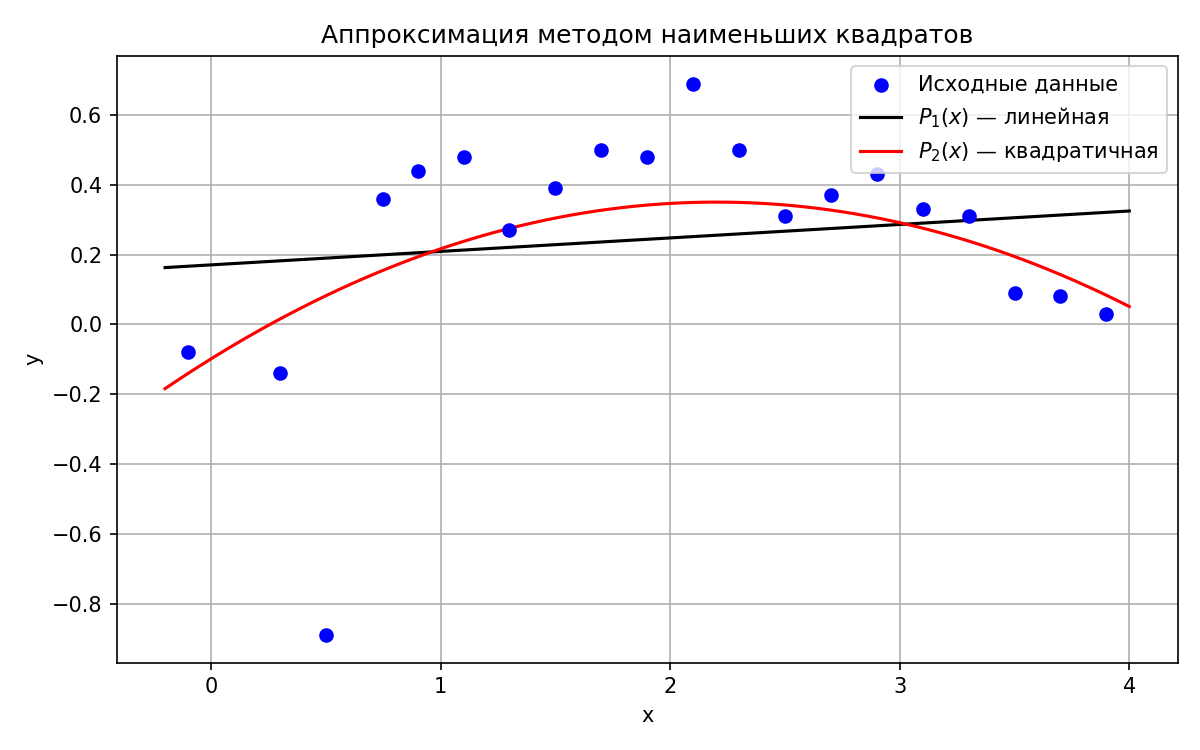
\includegraphics[width=0.8\textwidth]{pct/approximation.png}
    \caption{Графики исходных данных и аппроксимирующих полиномов.}
    \label{fig:approx}
\end{figure}

\section*{Заключение}
В ходе выполнения лабораторной работы была изучена полиномиальная аппроксимация методом наименьших квадратов. По таблице из $n = 20$ узлов были построены два аппроксимирующих полинома.

Для линейной аппроксимации $P_1(x) = a_0 + a_1x$ нормальная система МНК была составлена и решена, в результате чего получены коэффициенты $a_0 = 0.1705$ и $a_1 = 0.0386$:
\[
P_1(x) = 0.1705 + 0.0386 x.
\]
Наилучшее среднеквадратическое отклонение составило $\delta^{(2)}(P_1) = 0.3034$.

Для квадратичной аппроксимации $P_2(x) = a_0 + a_1x + a_2x^2$ получены коэффициенты $a_0 = -0.0988$, $a_1 = 0.4079$, $a_2 = -0.0926$:
\[
P_2(x) = -0.0988 + 0.4079 x - 0.0926 x^2.
\]
Наилучшее среднеквадратическое отклонение составило $\delta^{(2)}(P_2) = 0.2533$.

Квадратичная модель точнее линейной: $\delta^{(2)}(P_2) < \delta^{(2)}(P_1)$. Это закономерно, поскольку полином более высокой степени обладает большей гибкостью при подгонке к данным. Все вычисления выполнены программно на языке Python с использованием библиотеки NumPy.
